\chapter{Introduction} \label{ch:introduction}

This book is about directional extensions in Chadic languages. There are over 200 Chadic languages spoken across Nigeria, Cameroon and Chad. They make up the largest family of the Afroasiatic phylum. Many Chadic languages have complex verbal morphology. In descriptions of Chadic languages (and African languages, in general) it is common to find the term \textit{extension} used to refer to verbal morphology that has a function other than person-marking or tense-aspect. An extension may be an affix, clitic or particle, as long as it is morphosyntactically dependent on the verb. Among the functions of verbal extensions in Chadic languages, it is common to find extensions that mark whether a motion event described by the predicate involves a figure moving farther away or closer (as in \ref{ex:gizi1}), upward or downward (as in \ref{ex:huba3b}), inward or outward (as in \ref{ex:bura1}), and so on. These functions are described as \textit{directional}. Verbal extensions in Chadic languages which can express directional meaning are the focus of the research presented in this book.\footnote{The terms \textit{function} and \textit{meaning} are used interchangeably.} 

\ea\label{ex:gizi1}
\langinfo{\hyperref[gizi]{Giziga} verb \textit{kl} `run' with ventive suffix}{}{\cite[205]{shayGrammarGizigaChadic2021}} \\
\gll kl-ó	\\
run-\gl{vent} \\
\glt `Come running (over here)!'

\ex\label{ex:huba3b}
\langinfo{\hyperref[huba]{Huba} verb \textit{fəl} `jump' with downward suffix}{}{\cite[108]{muazuGrammarKilbaLanguage2009}} \\
\gll fəl-yà \\
jump-\gl{down} \\
\glt `to jump down'

\ex\label{ex:bura1}
\langinfo{\hyperref[bura]{Bura} verb \textit{nkya} `swim' with outward suffix}{}{\cite[274]{hoffmannUntersuchungenZurStruktur1955}} \\
\gll nkya-bila \\
swim-\gl{out} \\
\glt `swim out' [German: `\textit{hinausschwimmen}']
\z

There are several reasons for publishing this book. One is to refine the state of description of Chadic languages while providing a framework for more consistent and detailed morphosyntactic description in the future. A related goal is to advance comparative research on the grammars of Chadic languages with a study of unprecedented breadth and scope for this language family. As Chadic languages are by far the least-studied family within Afroasiatic, making progress toward a reliable typology of Chadic languages is foundational to gaining any new insights into the diverse and widespread Afroasiatic language phylum. Finally, within the domain of research on motion in grammar, this book offers a fresh look at multi-functionality in directional morphology and the complex relationships between verbs and directional verbal morphology.  

In this introductory chapter, Section \ref{sec:Chadic} is an introduction to Chadic languages in the context of research on Afroasiatic languages. Section \ref{sec:comparing} succinctly introduces the basic theoretical assumptions behind the approach to comparing languages assumed in this book. Section \ref{sec:motion} is a brief discussion of the larger context of research on motion in linguistics. Section \ref{sec:overview} provides an overview of the remaining chapters. 

\section{Chadic and Afroasiatic} \label{sec:Chadic}

The classification of Chadic languages used in this work is based on Glottolog 5.0 \citep{hammarstromGlottolog502024}. In this classification, there are 210 Chadic languages spoken across Nigeria, Cameroon and Chad.\footnote{The 28th edition of the Ethnologue lists 206 Chadic languages \citep{eberhardEthnologueLanguagesWorld2025}, slightly higher than the 196 Chadic languages that were listed in the 27th edition \citep{eberhardEthnologueLanguagesWorld2024}.} Together they make up the largest family in the Afroasiatic phylum (55\% of 381 total Afroasiatic languages). The history, validity and nomenclature of the Chadic family are discussed in \citet{porkhomovskyAfroAsiaticOverview2020}.\footnote{Note that the adjective \textit{Chadic} refers to the language family, and the adjective \textit{Chadian} refers to the country of Chad. Most Chadic languages are spoken outside of the Republic of Chad. Both the country and the language family are named after Lake Chad.}  

\begin{figure}
	\begin{forest}
		forked edges, for tree={edge=thick, s sep=-3pt, anchor=base west,  font=\strut\large, grow'=east} % s sep=0pt,
		[Chadic (210)
        [West Chadic (84)
        [A (38), tier=language]
        [B (46), tier=language]
        ]
        [Biu-Mandara (80)
		[Hurza (2), tier=language]
		[North (50), tier=language]
		[South (27), tier=language]
        ]
        [Masa (10)
        [North (6), tier=language]
        [South (4), tier=language]
        ]
        [East (36)
        [A: Chari-Logone (14), tier=language]
        [B: Guéra (22), tier=language]
        ]
        ]
	\end{forest}
	\caption{Internal classification of Chadic (Number of languages)} \label{fig:Chadic}
\end{figure}

\begin{figure}
	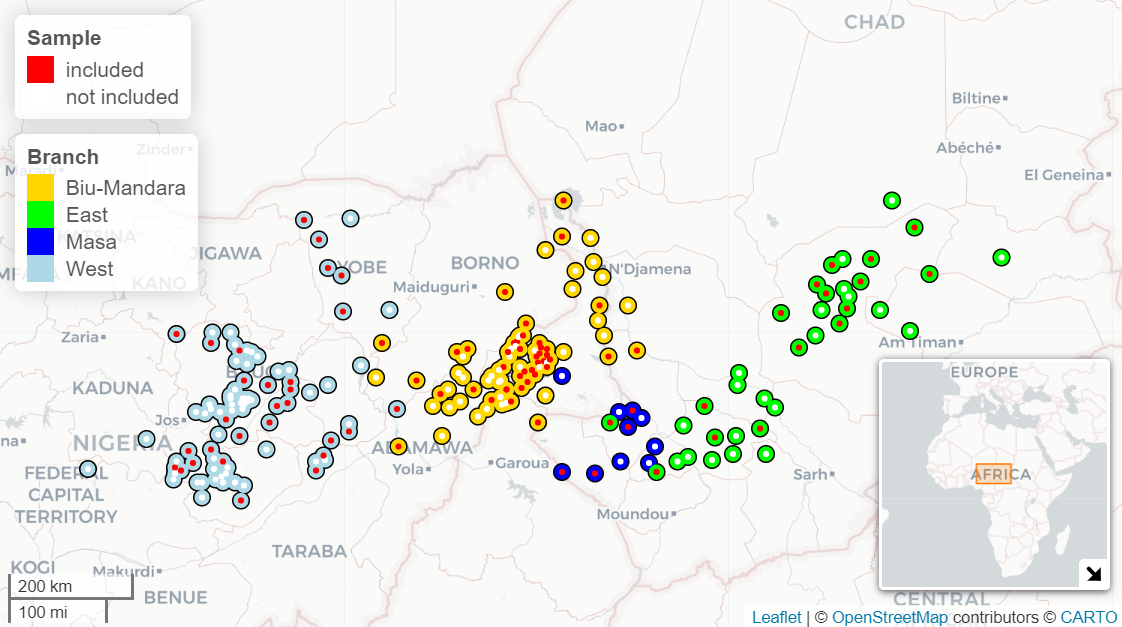
\includegraphics[width=\textwidth]{maps/Chadic.png}
	\caption{Map of Chadic languages based on Glottolog 5.0} \label{map:Chadic}
\end{figure}

The Chadic family is divided into four branches: West, Biu-Mandara, Masa, and East, as illustrated in Figure \ref{fig:Chadic} \citep{newmanComparativeChadicPhonology1966}.\footnote{One severely endangered Biu-Mandara language, Jilbe, has not been assigned to a subbranch of Biu-Mandara.} The geographic distribution of Chadic languages is shown in Figure \ref{map:Chadic}. The 84 West Chadic languages are spoken in the northeastern quadrant of Nigeria. The 80 Biu-Mandara languages (also known as Central Chadic) are spoken in a geographic area spreading across the Far North Region of Cameroon (\textit{Région de l'Extrême-Nord}) and extending westward over the Mandara mountains crossing the Nigerian border and eastward over the Chadian border. There are just ten Masa languages. They are geographically clustered around the southwestern part of Chad near the Cameroonian border. The 36 East Chadic languages are all spoken in the country of Chad.

The main issue of internal classification of Chadic languages has been the status of the Masa languages. \citet{shryockClassificationMasaGroup1997} summarizes the various perspectives on whether the Masa languages should be joined in a single branch with Biu-Mandara, or separated out at the branch level distinct from Biu-Mandara languages. He argues that Masa languages are a separate branch, based on phonological and lexical innovations which only occurred in the (non-Masa) Biu-Mandara languages, concluding that ``there is no conclusive evidence from shared innovations which supports the subclassification of the Masa group of languages in Biu-Mandara'' \citep[45]{shryockClassificationMasaGroup1997}. 

Studies of Chadic languages are mostly of fairly recent production. Only 14\% of the references on Chadic languages listed by Glottolog were published before 1960. There was a peak of publishing activity in the 1990s and early 2000s, as shown in Figure \ref{fig:publications}. This period of increased scholarly work on Chadic languages is all the more remarkable given the recurrent issues of restricted access due to periods of political instability in the region. In the last two decades there has been a decline in the number of publications on Chadic languages. This may be partially explained by a delay in incorporating recent publications into Glottolog's database, but it also coincidences with the retirement of a cohort of prominent Chadicists alongside very little evidence of continued institutional support for the study of African languages.

\begin{figure}
	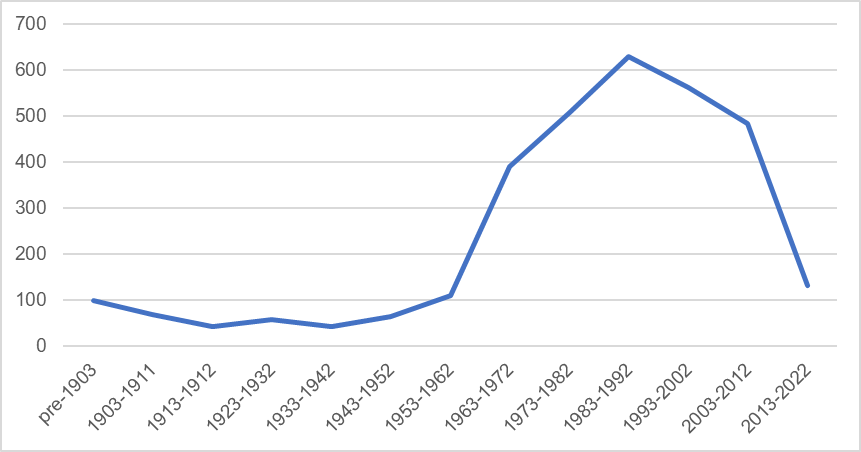
\includegraphics[width=\textwidth]{figures/publications.png}
	\caption{Number of publications on Chadic languages by decade} \label{fig:publications}
\end{figure}

In addition to publishing grammatical description of many Chadic languages, several authors have also published comparative overviews of the language family. Most of these are short summaries based on the author's own impression of general trends in the literature with clear bias toward languages that the author had firsthand experience studying \citep{newmanChadicLanguages2003,schuhChadicOverview2003,frajzyngierChadic2012,jaggarChadicLanguages2006,creisselsAfricaMorphosyntacticArea2008,jungraithmayrChadic2012,wolffChadicLanguages2014,caronChadic2020}.

The most substantial typological publication on Chadic languages is the unfinished work of \citet{schuhChadicCornucopia2017}, published posthumously. Schuh takes a historical-comparative approach, blending synchronic and diachronic analysis, and frequently proposing reconstructed forms based on a small sample of languages. By Schuh’s own admission, his work is somewhat biased toward the West Chadic languages he studied, and he had limited access to descriptions of East Chadic languages. Schuh’s overview of Chadic is illustrated by a small number of selected languages, and does not give a quantitative overview of how grammatical features are distributed among Chadic languages. It therefore remains uncertain how precisely Schuh's observations characterize Chadic languages as a family. 

The analysis of Chadic directional extensions in this book builds on the foundation of previous grammatical descriptions and typological generalizations. It provides a more precise quantitative approach to studying the distribution of grammatical features across Chadic languages. The intent is to align Chadic linguistics with typology in the sense of \citet[6]{bickelTypology21stCentury2007} who characterizes it as ``a discipline that develops variables for capturing cross-linguistic similarities and differences (qualitative typology), explores universal and local skewings in the distribution of these variables (quantitative typology) and proposes theories that explain the skewings (theoretical typology).''

By approaching the topic of motion in the grammar of Chadic languages from the perspective of modern typology, this work also provides a countermeasure to the relative lack of research being done on Chadic languages within Afroasiatic scholarship. Anecdotally, an online search of the contents of \textit{Brill's Journal of Afroasiatic Languages and Linguistics} brings up only four articles on Chadic languages in the 15 years since the inception of the journal in 2009. Using references in the Glottolog bibliography \citep{hammarstromGlottolog502024} as a measure of how thoroughly each language family has been studied, Ancient Egyptian is by far the most well-studied family with 254 references for just two languages. Three families have similar average numbers of references per language: Berber, 42.6; Cushitic, 47.4; Semitic, 39.2. The average number of references per language is much lower for Chadic languages at just 15.2.

Even for linguists with a more narrow focus on another family of Afroasiatic languages, parallel work on Chadic languages can provide crucial insights. As a relevant example of this, \citet[133]{fixSemanticsSemiticVentive2020} reviews over a century of studies of the ventive form of Akkadian verbs, including the work of no less than 30 scholars, concluding that: ``The reality is that despite some advances in terminology and categorization of ventive uses... the discussion of the Akkadian ventive has not actually progressed much from where Landsberger originally brought us with his [1924] article.'' The considerable effort given to the study of a single morphological form in a single extinct language did not prove to be a particularly fruitful approach. \citet[]{fixSemanticsSemiticVentive2020} instead proposes an approach that relies on insights from cross-linguistic studies. This book on directional extensions (including ventive forms) in Chadic languages provides a robust comparative picture of this topic, particularly from an Afroasiatic perspective. 

In addition, it is hoped that this work might kindle interest in the linguistic knowledge and creativity of the speakers of hundreds of understudied Afroasiatic languages spread across Africa. While there has been notable progress in describing and documenting Chadic languages, the reality is that the majority of Chadic languages have only minimal documentation, and many have never been studied. In some cases, their existence has only recently been documented \citep{blenchFiveUnexpectedChadic2016,blenchNewApproachesWest2017}. The opportunity to learn about Chadic languages may only be for a limited period of time, as speakers of the world's minoritized languages are under continual pressure to abandon their heritage languages leading to loss of linguistic knowledge within a few generations \citep{bromhamGlobalPredictorsLanguage2021,campbellNewKnowledgeFindings2013,simonsTwoCenturiesSpreading2019}.

\section{Comparing multi-functional morphemes} \label{sec:comparing}

As is now common practice in comparative linguistics (or typology), the concept of \textit{directional extensions} as applied in this cross-linguistic study is proposed as a \textit{comparative concept}, constructed by a linguist for the purpose of comparing linguistic systems, and not a \textit{cross-linguistic category}, a kind of naturally occurring entity that can be diagnosed as having the same set of properties across languages \citep{haspelmathPreestablishedCategoriesDont2007, haspelmathComparativeConceptsDescriptive2010}. Even very similar morphemes in different languages are not assumed to be identical in their morphosyntactic and semantic properties. For example, identifying morphemes in different languages as meeting the definition of \textit{ventive extensions} (as a comparative concept) does not entail that those morphemes will have the same range of functions, the same morphosyntactic distribution, or the same diachronic development. 

Given that directional extensions have not been central to theories of universal linguistic structures, there are no unnecessary controversies to unravel regarding the status of directionals as a cross-linguistic category. However, a linguist describing a particular language may find that the comparative concepts used in this book do not capture the particularities of that language's verbal morphology in a natural or insightful manner. This is unproblematic because comparative concepts are distinct from language-particular categories. 

For example, the West Chadic language \hyperref[kana]{Kanakuru} has two morphemes which meet the definition of the comparative concept \textit{ventive direction extension} described in Chapter \ref{ch:identifying}. One is a verbal suffix \textit{-tə(ru)} and the other is a preverbal particle \textit{bo}. Naturally, \citet{newmanKanakuruLanguage1974} distinguishes these forms, describing one as a ``ventive suffix'' and the other as a ``ventive equivalent auxiliary''. From a cross-linguistic perspective, it is noteworthy that this is the only example of a pre-verbal directional extension in the data. At the same time, it would not be worth refining the comparative concept to distinguish pre-verbal and post-verbal extensions for one outlier in the data. Therefore, the two distinct morphemes in Kanakuru are both treated as ventive extensions in regard to cross-linguistic generalizations.

While \textit{directional extension} as a comparative concept is narrowly defined without regard to the full semantic profile of each morpheme, the multi-functionality of directional extensions is not being ignored. Rather, a fundamental contribution of this research project is to provide a quantitative analysis of multi-functional morphemes. Once a set of verbal extensions with directional semantics is identified, it is then possible to ask what other functions these same forms have. The term ``co-expression'' is used to described ``the relation between a linguistic form in a given language and several functions that are expressed by different forms in some other language'' \citep[476]{hartmannIdentifyingSemanticRole2016}. 

For example, in \hyperref[huba]{Huba}, the same verbal extension that expresses downward direction in one context (in \ref{ex:huba3b} above) can express completive aspect in another context, as in (\ref{ex:huba02b}). In contrast, in most languages, aspectual meanings like completive are expressed by forms distinct from morphemes that express downward direction. Therefore, this one form in Huba is considered to co-express (at least) two functions. Nonetheless, the suffix \textit{-yà} is considered a directional extension because it has a directional function in (\ref{ex:huba3b}), irrespective of what functions it may co-express.

\ea\label{ex:huba02b}
\langinfo{\hyperref[huba]{Huba} verb \textit{wùr} `finish' with downward suffix}{}{\cite[108]{muazuGrammarKilbaLanguage2009}} \\
\gll wùr-yà	\\
finish-\gl{down}	\\
\glt `to finish completely'
\z 

\section{Motion in grammar} \label{sec:motion}

The universality, salience and complexity of motion in grammar has held the attention of linguists for decades. Motion entails a conceptualization of both space and time. Much of the work on motion in language has had an aim of gaining insights into human cognition by comparing how people from different cultures and languages might think differently about space and time. For example, well-known work of \citet{levinsonSpaceLanguageCognition2003} and \citet{levinsonGrammarsSpaceExplorations2006} highlights the diverse frames of reference (intrinsic, relative, absolute) applied to descriptions of location and motion, as well as the the diversity of how frame of reference is encoded in linguistic structures. They discuss how speakers of languages with grammaticalized forms for expressing cardinal directions are consistently able to identify cardinal directions and to recall the cardinal orientation of past events. Other researchers have focused on the morphosyntactic representation of the source and goal of motion events in adpositions and case marking or in adverbial interrogatives and demonstratives \citep{creisselsEncodingDistinctionLocation2006, kopeckaSourcegoalAsymmetriesLanguages2021, nintemannHereHitherHence2020, stolzCrosslinguisticsZeromarkingSpatial2014, stolzSpatialInterrogativesEurope2017}.

Much of the terminology commonly found in descriptive and comparative studies of motion events is drawn from the work of \citet{talmyLexicalizationPatternsSemantic1985}  \citep[see also][25--26]{talmyCognitiveSemantics2000}. Motion events exclude self-contained (or non-translational) motion, as in \textit{The log rolled over and over in water}, but include stationary (or stative) location. In a motion event, a person or object (the figure) is described as maintaining or changing location relative to some other entity (the ground). If the location changes (translational motion), the characterization of how the position of the figure changes with respect to the ground is known as the path of motion. 

Generally, linguistic expressions describing a change of location do not include a precise, detailed retracing of the geometry of the path of motion, but will rather reference a few relevant aspects of the path of motion. The description of the path might only give a single point of reference, for example, away from a source or towards a goal. The source or goal of the path may be identified with the notion of a deictic center: a fixed point of reference typically corresponding to the location of the speaker, as in `here'. More complex geometric notions can also be included in the description of the path of motion. For example, a boundary-crossing path is defined in reference to a bounded space (e.g., \textit{into a house} or \textit{out of a box}).%\footnote{\citet[53]{talmyCognitiveSemantics2000} refers to these components of describing a path of motion as ``Vector'', ``Deictic'' and ``Conformation''.}

Semantic content defining the path of motion can be included in the meaning of a motion verb. For example, the motion interpretation of the English verb \textit{enter} in the phrase \textit{They entered the house} entails that a figure (referenced by the subject) moves along a path of motion which begins outside of a bounded space (`the house') and crosses the boundary to an endpoint within the bounded space. It is also common for a verb of motion to be modified by some other morpheme which adds details about the path of motion. For example, the English preposition \textit{into} has a meaning similar to the verb \textit{enter}. The preposition can be combined with a generic motion verb as in \textit{move into the circle} to express an inward path of motion without the direction being defined by the verb itself.

\citet{talmyPathRealizationTypology1991} created a dichotomous typology by distinguishing cases where information about the path of motion is expressed by the main verb of a clause from all other possible ways of expressing a path of motion. In this approach, linguistic expressions of motion events are either ``verb-framed'' (the path is expressed by the main verb) or ``satellite-framed'' (the path is expressed elsewhere).\footnote{Talmy's original typology focused on categorizing language types. However, most languages allow for more than one way to express the path of motion, and so a typology of language types relies on an assessment of speakers' or signers' general tendencies when using the language. This rather vaguely defined notion was later made more precise by researchers who applied these concepts to describing types of linguistic expressions or grammatical constructions rather than types of languages \citep[e.g.][]{beaversTypologyMotionExpressions2010,croftRevisingTalmyTypological2010}.} Under Talmy's approach, ``satellites'' would include verbal morphology, adverbial expressions and subordinate verbs \citep[103]{talmyCognitiveSemantics2000}.\footnote{Talmy argues that even in the case of serial verb constructions where the syntactic relationship between the verbs in a clause does not have the grammatical properties typically associated with subordination it should, in principle, be possible to identify one of the verbs in the construction as the main verb and the other as a satellite \citep{talmyPropertiesMainVerbs2016}.}

Chapter \ref{ch:verbs} takes an alternate perspective on Talmy's typology of the expression of the directional meaning. Rather than examining speakers' preferences for choosing between forms which express directional meaning in the verb (verb-framed) or elsewhere (satellite-framed), this chapter looks at the availability of expressing direction either in the root of a motion verb or as a verbal extension. For certain types of direction, there is a pattern of complementary distribution within the verbal complex such that the direction is either lexicalized in the verb root or grammaticalized in the verbal morphology, but not both. This can be viewed as a type of efficiency in the grammar, avoiding redundant expression of the same meaning in multiple forms. However, for ventive and itive directional meaning, redundancy is more common than complementary distribution. 

While the research presented in this book relies on Talmy's conceptual and terminological work, it is not a Talmian typological analysis of the expression of motion in verbs and satellites. The starting point is not how the elements of motion are expressed across syntactic constructions, but rather the expression of path of motion in the verbal extensions. This set of morphemes is narrower than the broad concept of satellites. It does not include adverbs, subordinate verbs or serial verb constructions. Semantically, the primary interest in this work is the limited number of directional meanings that are frequently expressed in verbal extensions in Chadic languages.\footnote{The expression of these directional meanings in verb roots is discussed in Chapter \ref{ch:verbs}.}
 
Directional semantics have been included as an element of many previous typological studies; however, there has not been a particular focus on directional verbal morphology until recently. It was in the process of studying associated motion\index{associated motion} morphology that several authors noted the need to distinguish directional morphemes from associated motion, leading to the topic of directional morphology receiving more attention in its own right \citep{bourdinMarkingDirectionalDeixis2006,belkadiAssociatedMotionDeictic2015,guillaumeAssociatedMotionSouth2016}. It is in the context of discussing associated motion that \citet{rossCrosslinguisticSurveyAssociated2021,rossPseudocoordinationSerialVerb2021} provides a global cross-linguistic quantitative study of directional verbal morphology. Part of the research presented in this book contains a study similar to \citet{rossCrosslinguisticSurveyAssociated2021} but focused on Chadic languages (Chapters \ref{ch:identifying}, \ref{ch:identifying2} and \ref{ch:distribution}).

One of the particular areas of interest in the typology of directional verbal morphology has been the co-expression of associated motion\index{associated motion} with directionality \citep{dryerAssociatedMotionDirectionals2021,belkadiDeicticDirectionalityAssociated2021}. An example of this can be seen in \hyperref[zulg]{Zulgo-Gemzek} where the verbal extension \textit{-áha} can have a directional function (itive) with a motion verb, as in (\ref{ex:zulg4}), but can also have a subsequent associated motion meaning with a non-motion verb, as in (\ref{ex:zulg6b}). The crucial distinction is that in (\ref{ex:zulg6b}), the meaning of the verb does not entail any motion -- the motion event is due to the presence of the verbal extension. 

\ea\label{ex:zulg4}
\langinfo{\hyperref[zulg]{Zulgo} verb \textit{val} `run' with itive suffix}{}{\cite[47]{hallerVerbalComplexZulgo1981}} \\
\gll á-val-áha \\
he-ran-\gl{itive} \\
\glt `He ran there.'

\ex\label{ex:zulg6b}
\langinfo{\hyperref[zulg]{Zulgo} verb \textit{zə́m} `eat' with itive suffix}{}{\cite[47]{hallerVerbalComplexZulgo1981}} \\
\gll á-zə́m-áha daf \\
he-ate-\gl{itive} fufu \\
\glt `He ate fufu and went there.'
\z 

This issue is explored for Chadic languages in Chapters \ref{ch:functions} and \ref{ch:interpretation}. The database created for this research (Chapter \ref{ch:identifying2}, Section \ref{sec:database}) tracks what meanings are co-expressed with directional meaning, including associated motion\index{associated motion}, allowing a quantitative approach to studying the multi-functionality of motion morphology (Chapter \ref{ch:functions}) including which meanings occur with what verb roots (Chapter \ref{ch:interpretation}).

Another domain of motion research in linguistics that has recently been given more attention is the expression of bringing and taking events, which \citet{margettsCausedAccompaniedMotion2022} call \textit{directed caused accompanied motion} (directed CAM). Chapter \ref{ch:CAM} contributes to this relatively new area of focus by presenting a distributional typology of directed CAM in Chadic languages. 

Finally, this book contributes to the empirical study of motion in language by improving the state of art in the description of Chadic languages. The appendices present a brief description of the directional verbal morphology and other related aspects of 91 Chadic languages. A major aim of this book is to provide a tool that helps linguists have more appropriate concepts and vocabulary for understanding and describing the expression of motion in the grammars Chadic languages, thus contributing to the ``persistent need to document expressions of spatial relations and motion events in natural languages'' \citep[14]{robbersOrientationMotionWorld2023}. 

\section{Overview of this book} \label{sec:overview}

The remainder of this book is divided into seven core chapters followed by a brief summary chapter. Chapter \ref{ch:identifying} defines and exemplifies the semantic subtypes of directional extensions found across Chadic languages. Chapter \ref{ch:identifying2} is closely related in that it provides further clarification on how particular linguistic examples were classified, dealing with many-to-one and one-to-many form-function relationships as well as some borderline cases of motion events. This chapter also discusses the implications of these analytical choices for the database used in the quantitative analyses throughout this book.

Chapter \ref{ch:distribution} presents the results of the first quantitative study: how frequently each type of directional extension is found across the 91 Chadic languages included in this research. The most common type is ventive meaning, but among the Biu-Mandara languages many other types of directional meaning are found expressed in verbal extensions. The final section looks at what types of directional extensions co-occur in each language. Although ventive is the most common type, there is no (synchronic) implicational hierarchy that predicts the existence of a ventive directional extension in languages with more than two directional extensions. 

Chapter \ref{ch:diachrony} covers the diachrony of directional extensions in Chadic languages. Naturally, the synchronic comparative data raises questions about the history of these forms that led to their current distribution across Chadic languages. While no particular directional extensions can be reconstructed to a Proto-Chadic form, there are some general patterns that allow some basic hypotheses to be formed. Ventive directional extensions can be plausibly reconstructed for West Chadic languages, but it is uncertain that these forms share a historical relationship with ventive directional extensions in other branches. Most other types of directional extensions have only developed in Biu-Mandara languages and their forms suggest multiple innovations from various sources in different languages.

Chapter \ref{ch:verbs} examines patterns of efficiency and redundancy in grammatical systems by comparing the distribution of directional meaning in verbal extensions with the distribution of the same meaning in verb stems (i.e., directional verbs) in Chadic languages. The results show that vertical (upward, downward) and boundary-crossing (inward, outward) directional meanings have a strong tendency to occur in complementary distribution. Languages with vertical or boundary-crossing directional extensions rarely have these same meanings expressed by vertical or boundary-crossing directional verbs, and vice versa. The same is not true of ventive and itive extensions. These meanings are often redundantly expressed in both a verbal extension and in a verb stem. However, there is a correlation between the presence of a ventive directional extension and having a general motion verb (unspecified for direction). 

Chapter \ref{ch:functions} is an analysis of the non-directional functions co-expressed by directional extensions, including how frequently various functions are co-expressed with each type of directional meaning across the 91 languages in the sample. The most commonly reported meanings co-expressed with directional meaning in verbal extensions are other types of motion or location meaning, especially subsequent associated motion\index{associated motion}. In addition to these functions, a directional extension may lexicalize in combination with a particular verb to express an idiomatic or non-compositional predicate meaning, much like phrasal verbs in English. It is also commonly reported that directional extensions co-express an aspectual meaning or have other grammaticalized, non-motion functions; however, such claims are often made without the support of clear contrastive evidence from language data.  

Chapter \ref{ch:interpretation} expands on the study of co-expression of various meanings in verbal extensions to examine whether the lexical semantics of the verb stem is predictive of the interpretation of the verbal extension. As expected, a verbal extension that can express directional meaning nearly always does so when modifiying a motion verb, but this is not without exceptions. A number of verbs, such as verbs of hitting or removing, are not typical motion verbs but can be construed as happening along a path of motion when combined with a directional extension. However, verbal extensions combined with the same verbs are also frequently given other motion-related interpretations (such as subsequent or resultative motion). Overall, the conclusion is that the lexical semantics of the verb may correlate with a particular interpretation of a directional extension, but the meaning of the verb on its own does not fully determine how the verbal extension will be interpreted. 

Chapter \ref{ch:CAM} is the first of two chapters that take a broader perspective on directional extensions in Chadic languages by selecting a particular semantic domain (or function) in which directional extensions are frequently found, and then comparing how that semantic domain is linguistically structured across Chadic languages. The first domain examined is directed caused accompanied motion (CAM), as in the English verb `bring'. One of the two most frequent ways of expressing directed CAM is to combine a verb of possession, e.g., `take', with a directional extension. It is slightly more common to find directed CAM expressed by a directional verb with valency-increasing morphology. It is argued that both of these forms are lexicalized or idiomatic expressions of directed CAM, contrary to previous approaches that assume they can be synchronically parsed (i.e., semantically decomposed) maintaining a standard directional or causative interpretation of the verbal morphology. 

\largerpage
Chapter \ref{ch:buysell} presents a second semantic domain in which directional extensions are commonly found in Chadic languages: the distinction between the notions `buy' and `sell'. These notions differ only in regard to whether the primary argument is the one giving or receiving money in the transaction -- a distinction that would only have become relevant millenia after the Chadic languages began to spread across the Sahel region. In order to make this distinction, many Chadic languages have borrowed a verb for `sell' or extended the meaning of another verb to express `sell'. It is also common to find languages with a verb that can be translated as either `buy' or `sell' but which can take additional verbal morphology to make the distinction explicit. This morphology is typically either a directional extension or a valency-increasing morpheme. Which form is used (including which directional path is used in the case of directional extensions) is not predictable from language to language. This indicates that these are lexicalized verb-extension combinations created to fill the functional need that arose with the introduction of currency. 

\largerpage
Chapter \ref{ch:summary} is a brief summary. This is followed by an extended appendix which presents the analysis of the relevant data for each of the 91 languages included in this study. Throughout this book, the names of languages in the sample are hyperlinked to the section in the appendix that gives an overview of the data for that language.

